\chapter{Niezmienniki izometrii}

\section{16.10.2024}{Końce (w nieskończoności) grup przestrzeni}

Zanim zaczniemy, zróbmy szybką motywację, czyli graf Cayleya grupy $\Z$ z jednym generatorem:
\begin{center}
  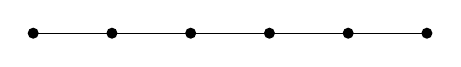
\begin{tikzpicture}
    \draw (0, 0)--(5, 0);
    \foreach \i in {0, 1, ..., 5} \fill (\i, 0) circle (2pt);
  \end{tikzpicture}
\end{center}
który ma "dwa końce". Natomiast grupa wolna $F_2$ o dwóch generatorach ma "nieskończenie wiele końców". 
\begin{center}
  \begin{tikzpicture}
    % \tikzmath {
    %   \power = 2.3;
    %   \numsteps = 4;
    %   \deviation = 90;
    %   function drawRec(\x, \y, \rotate, \step) {
    %     \step = \step - 1;
    %     if (\step >= 0) 
    %     then {
    %       \scale = \power^\step;
    %       \draw
    %       [
    %         shift={(\x pt,\y pt)},
    %         rotate=\rotate,
    %         scale=\scale,
    %         line width=\scale*.1 pt,
    %         line cap=round,
    %       ]
    %         (0,0)--(1,0) coordinate (newbase);
    %       coordinate \b;
    %       \b1 = (newbase); % the new base point
    %
    %       for \a in {-\deviation,0,\deviation} {
    %         drawRec(\bx1,\by1,mod(\rotate+\a,360),\step); % draw one child edge
    %       };
    %     };
    %   };
    %   for \angle in {0,90,180,-90} {
    %     drawRec(0,0,\angle,\numsteps);
    %   };
    % }
    \tikzmath {
    }
  \end{tikzpicture}
\end{center}
Z drugiej strony, grupa $\Z^2$ ma jeden koniec: jeśli weźmiemy dwa bardzo odległe od siebie obszary, to one są ze sobą połączone, chociaż jest to połączenie "bardzo odległe".
\begin{center}
  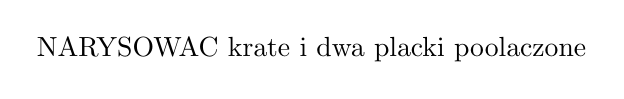
\begin{tikzpicture}
    \node at (0,0) {NARYSOWAC krate i dwa placki poolaczone};
  \end{tikzpicture}
\end{center}
Z kolei każda przestrzeń skończona, np. graf Cayleya grupy skończonej, ma $0$ końców.

\subsection{Podejście przez granice}

\begin{definition}{zbiór skierowany}{}
  Zbór z częściowym proządkiem $(\Lambda, \leq)$ jest \buff{skierowany}, gdy dla dowolnych $\lambda_1,\lambda_2\in\Lambda$ istnieje $\lambda\in\Lambda$ takie, że $\lambda\geq \lambda_1$ oraz $\lambda\geq \lambda_2$.
\end{definition}

{\large\color{red}ciągi odwrotne}

\begin{definition}{system odwrotny}{}
  \buff{System odwrotny} nad zbiorem skierowanym $\Lambda$ to rodzina zbiorów 
  $$\mathfrak{X}:=\{X_\lambda\;:\;\lambda\in\Lambda \}$$
  oraz rodzina odwzorowań
  $$\mathcal{F}:=\{f_{\lambda\mu}:X_\mu\to X_\lambda\;:\;\lambda\leq\mu \}$$
  takich, że 
  \begin{enumerate}
    \item dla dowolnego $\lambda$ mamy funkcję identycznościową: $f_{\lambda\lambda}=id_{X_\lambda}$
    \item dla dowolnych $\lambda\leq\mu\leq\nu$ złożenia zachowują się dobrze: $f_{\lambda\nu}=f_{\lambda\mu}\circ f_{\mu\nu}$.
  \end{enumerate}
\end{definition}

Będziemy oznaczać: $\boldsymbol{\underline{X}:=(\Lambda, \mathfrak{X}, \mathcal{F})}$

\begin{definition}{granica odwrotna}{}
  Granicą odwrotną systemu $\underline{X}$ nazywamy zbiór
  $$\underset{\leftarrow}{\lim}=\{\xi\in\prod_{\lambda\in\Lambda}X_\lambda\;:\;(\forall\;\lambda'\leq\lambda)\;\xi_{\lambda'}=f_{\lambda'\lambda}(\xi_\lambda)\}.$$
  Elementy $\xi$ jak wyżej nazywamy \hl{niciami} (threads) w $\underline{X}$.
\end{definition}

\begin{definition}{odwzorowania graniczne}{}
  Odwzorowania 
  $$f_\lambda:\varprojlim\underline{X}\to X_\lambda$$ 
  takie, że $f_\lambda(\xi)=\xi_\lambda$ nazywamy odwzorowaniami granicznymi.
\end{definition}

O odwzorowaniach granicznych można myśleć jako o odwzorowaniach, które pytają "kim byłem w czasie $\lambda$".

\begin{center}
  \begin{tikzcd}
    X_1 & X_2 \arrow[l] & X_3\arrow[l] & X_4 \arrow[l] & ... \arrow[l]\\ 
        & & \varprojlim\underline{X}\arrow[ull]\arrow[ul]\arrow[u]\arrow[ur]\arrow[urr]
  \end{tikzcd}
\end{center}

Dla $\lambda\leq\mu$ diagram 
\begin{center}
  \begin{tikzcd}
    &\underset{\leftarrow}{\lim}\underline{X}\arrow[dl, "f_\lambda"]\arrow[dr, "f_\mu"]\\ 
    X_\lambda && X_\mu\arrow[ll, "f_{\lambda\mu}"]
  \end{tikzcd}
\end{center}
zawsze komutuje.

\subsection{Toopologia granicy odwrotnej}

Kiedy zbiory $X_\lambda$ są przestrzeniami topologicznymi, zaś $f_{\lambda\mu}$ są ciągłe, to na granicy odwrotnej $\varprojlim\underline{X}$ rozważamy również topologię graniczną. Jest to topologia dziedziczona z topologii produktowej na $\prod_{\lambda\in\Lambda}X_\lambda$. \hl{Bazą tej topologii są zbiory postaci }\hl{$f_\lambda^{-1}(U)$ dla $\lambda\in\Lambda$ i otwartych $U\subseteq X$.}

\begin{fact}{}{}
  Gdy przestrzenie $X_\lambda$ są Hausdorffa, to $\varprojlim \underline{X}$ jest domkniętym podzbiorem w $\prod_{\lambda\in\Lambda}X_\lambda$.
\end{fact}

Gdy przestrzenie $X_\lambda$ są zwarte i metryczne, to wówczas $\varprojlim\underline{X}$ też jest zwarta i metryczna. W szczególności, gdy $X_\lambda$ są skończone (z topologią dyskretną), zaś $\Lambda$ jest przeliczalny, to wówczas $\varprojlim\underline{X}$ jest \hl{przestrzenią zwartą i metryczną}. Na ogół nie jest też przestrzenią dyskretną, mimo że wszystkie zbiory po których bierzemy granicę takie były (bazą topologii są przeciwobrazy punktów $\{\xi\in\varprojlim\underline{X}\;:\;\xi_\lambda=x\}=f^{-1}_\lambda(x)$).

\begin{example}{}{}
  Niech $\Lambda=(\N, \leq)$ i niech $X_k$ będzie zbiorem wszystkich ciągów $0-1$ długości $k$. Dla $k\leq m$ rozważamy 
  $$f_{km}:X_m\to X_k$$
  będące obcięciem ciągu długości $m$ do początkowego ciągu długości $k$. Dostajemy wówczas system odwrotny $\underline{X}=(\N, \{X_k\}, \{f_{km}\})$ zbiorów skończonych. Wówczas $\varprojlim\underline{X}$ jest homeomorficzny ze zbiorem Cantora.
\end{example}

Będziemy zajmować się $X$ które są przestrzeniami metrycznymi, geodezyjnymi właściwymi, np. grafami Cayleya grup skończenie generowanych. $\mathcal{K}$ to będzie rodzina wszystkich zwartych podzbiorów $K\subseteq X$ z porządkiem inkluzji.

\begin{definition}{podzbiór współkońcowy}{}
  Podzbiór $M\subseteq\Lambda$ zbioru skierowanego $\Lambda$ nazywamy \buff{współkońcowym}, jeśli 
  $$(\forall\;\lambda\in\Lambda)(\exists\;\mu\in M)\;\lambda\leq\mu,$$ 
  wtedy $(M, \leq)$ też jest zbiorem skierowanym. Dla $\underline{X}=(\Lambda, \mathfrak{X}, \mathcal{F})$ niech 
  $$\underline{X}_{|M}=(M, \{X_\lambda\;:\;\lambda\in M\}, \{f_{\mu\mu'}\in\mathcal{F}\;:\;\mu,\mu'\in M\})$$
  będzie obcięciem $\underline{X}$ do $M$. Wtedy $\underline{X}_{|M}$ jest systemem odwrotnym nad $M$.
\end{definition}

\begin{fact}{}{}
  $$\varprojlim\underline{X}=\varprojlim\underline{X}_{|M}$$
  Przez bijekcją polegającą na obcinaniu nici do $M$. Jest ona jednocześnie homomorfizmem.
\end{fact}

\begin{conclusion}{}{} 
  Jeśli $X_\lambda$ są zwarte i metryczne, zaś $\Lambda$ posiada przeliczalny podzbiór współkońcowy, to $\varprojlim\underline{X}$ jest zwarta i metryczna.
\end{conclusion}

\begin{example}[m]
  \item W przykładzie wyżej zbiór $\mathcal{K}$ posiada współkońcowy podciąg $K_i:=B_{i\cdot R}(x_0)$ dla $R>0$ i pewnego $x_0\in X$.
  \item Dalej używając oznaczeń z poprzedniego przykładu, dla dowolnego $K\in\mathcal{K}$ niech $\Pi_K^X$ będzie zbiorem nieograniczonych komponent spójności w dopełnieniu $X-K$.\medskip

    Przestrzeń geodezyjna jest lokalnie drogowo spójna. Każda jej otwarta podprzestrzeń również jest lokalnie drogowo spójna. Czyli każde $X-K$ też jest lokalnie drogowo spójna. W lokalnie drogowo spójnych przestrzeniach komponenty spójności to to samo co komponenty drogowej spójności.\medskip 

    Każda nieograniczona komponenta $C'\subseteq X-K'$ zawiera się w dokładnie jednej nieograniczonej komponencie $C\subseteq X-K$. Dostajemy odwzorowanie $f_{KK'}:\Pi_{K'}^X\to \Pi_K^X$ takie, że $f_{KK'}(C')=C$.\medskip
  
    Trójka $(\mathcal{K}, \{\Pi_K^X:K\in\mathcal{K}\}, \{f_{KK'}:K\subseteq K'\})$ tworzy system odwrotny nad zbiorem skierowanym $\mathcal{K}$.

    \begin{center}
      \begin{tikzcd}
        \Pi_K^X & \Pi_{K'}^X\arrow[l, "f_{KK'}"] & \Pi_{K''}^X\arrow[l, "f_{K'K''}"]
      \end{tikzcd}
    \end{center}

    \begin{fact}{}{}
      Dla każdego $K\in\mathcal{K}$ zbiór $\Pi_K^X$ jest skończony.
    \end{fact}

    \begin{proof}
      Weźmy $K\subseteq B_r(x_0)$, niech $R>r$ i rozważmy kulę $B_R(x_0)$, która jest zwarta. Każda nieograniczona komponenta $C$ spójności w $X-K$ przecina niepusto sferę $S_R(x_0)$, bo $X$ jest geodezyjna.

      Zatem przekrój $C\cap B_R(x_0)$ jest niepusty. Wtedy rodzina 
      $$\{C\cap B_R(x_0)\;:\;C\text{ dowolna komponenta dopełnienia }X-K\}\cup \{\overline{B_R}(x_0)=B_R(x_0)-S_R(x_0)\}$$
      pokrywa $B_R(x_0)$. Dodatkowo, jest to otwarte pokrycie, bo komponenty spójności lokalnie spójnej przestrzeni są otwartymi podzbiorami w tej przestrzeni. Ze zwartości $X$ to pokrycie posiada skończone podpokrycie, ale z drugiej strony każdy zbiór postaci $C\cap B_R(x_0)$ dla nieograniczonych komponent musi przetrwać w każdym podpokryciu, bo zawiera punkty które należą tylko do niego. Stąd nieograniczonych komponent jest skończenie wiele.
    \end{proof}
\end{example}

\begin{definition}{}{}
  Zbiorem (przestrzenią) końców, $Ends(X)$, właściwej geodezyjnej przestrzeni metrycznej $X$ nazywamy granicę odwrotną
  $$Ends(X)=\varprojlim(\Pi^X)=\varprojlim(\mathcal{X}, \{\Pi_K^X\}, \{f_{KK'}\}),$$
  gdzie $\Pi_K^X$ to nieograniczone komponenty w $X-K$.  Jest to zwarta przestrzeń metryczna.
\end{definition}



